\documentclass[dvipsnames,svgnames]{beamer}
\usetheme{Warsaw}
\usepackage[utf8]{inputenc}
\usepackage[english]{babel}
\usepackage{amsmath}
\usepackage{amsfonts}
\usepackage{amssymb}
\usepackage{graphicx}
\usepackage[linesnumbered,ruled]{algorithm2e}
\usepackage{tikz}
\usetikzlibrary{automata, positioning}
\usepackage{float}
\usepackage[normalem]{ulem}
\usepackage{color}
\usepackage{xcolor}

\expandafter\def\expandafter\insertshorttitle\expandafter{%
	\insertshorttitle\hfill%
    \insertframenumber\,/\,\inserttotalframenumber}



\author{Charles Dufour}
\title{Reinforcement learning and robot navigation }
%\setbeamercovered{transparent} 
\setbeamertemplate{navigation symbols}{} 
%\logo{} 
\institute{Supervisors: Prof. F. Eisenbrand, Jonas Racine} 
\date{June 20, 2018}
%\subject{} 

\newtheorem{madef}{Definition}

\begin{document}


\begin{frame}
\titlepage
\centering
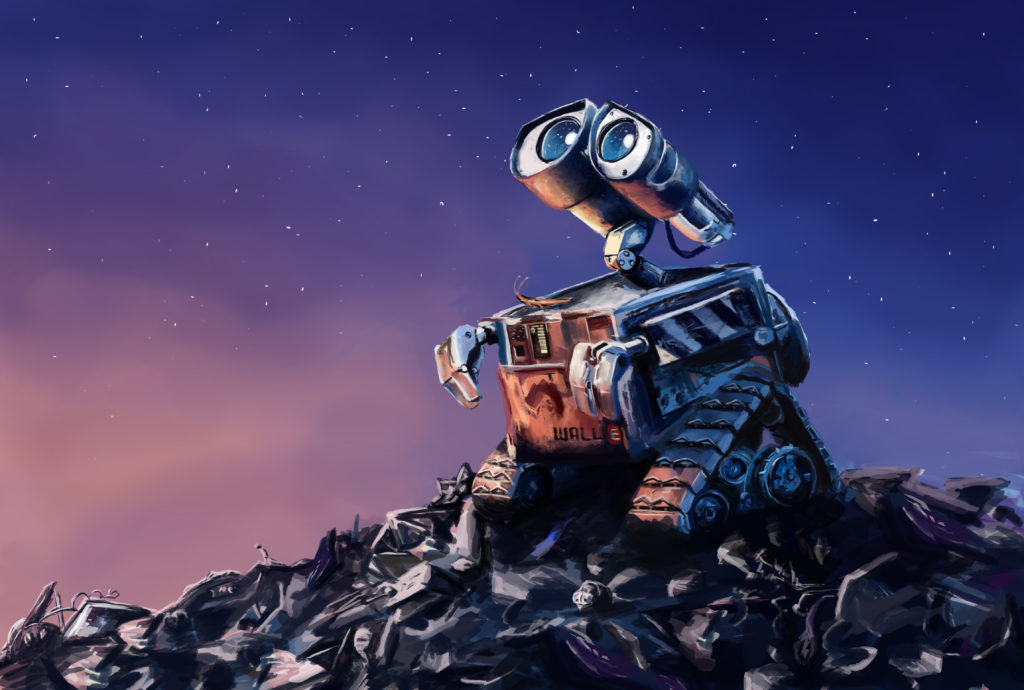
\includegraphics[scale=1]{img/Wall-E.jpg}
\end{frame}

%\begin{frame}
%\tableofcontents
%\end{frame}



\begin{frame}
\frametitle{Introduction}
\begin{block}{The problem}

  \begin{itemize}
   \item Framework: a raspberry pi 3 robot which can follow lines
   \item The task: the robot should adapt its speed with respect to traffic lights
   \item How: using Reinforcement Learning (RL) and Markov Decision Process (MDP)  
  \end{itemize}
\end{block} 
\end{frame}

\begin{frame}
\frametitle{The task}
\begin{center}
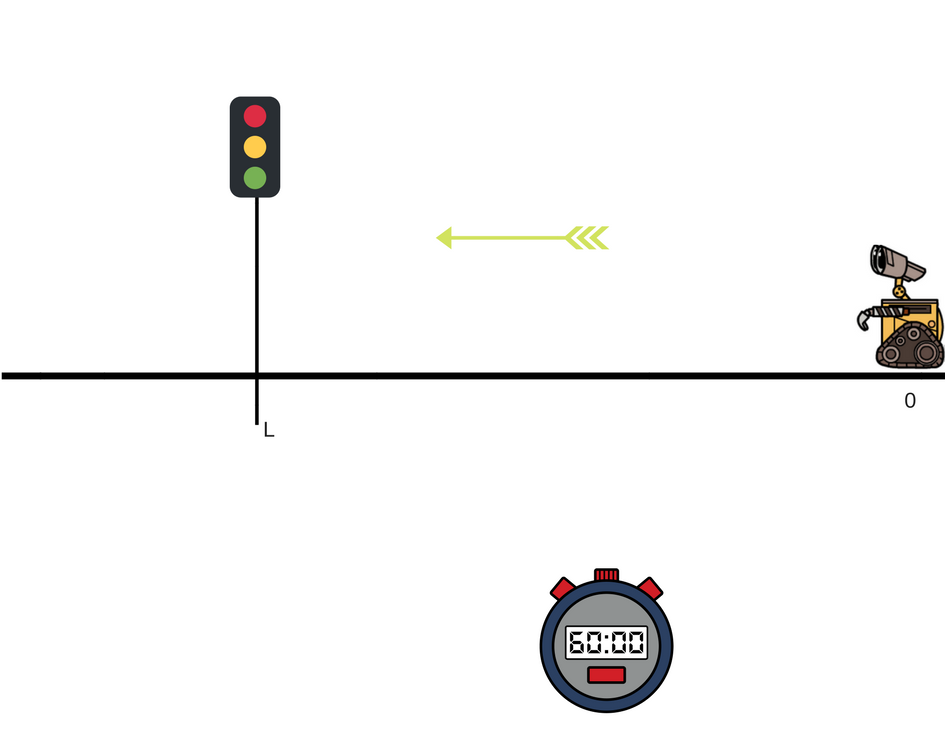
\includegraphics[scale=0.4]{img/illustration_traffic_light.png}
\end{center}
\end{frame}

\begin{frame}{Presentation}
\begin{block}{}
\begin{itemize}
\item Part I: theoretical background 
\item Part II: results from first implementations
\end{itemize}
\end{block}
\end{frame}

\begin{frame}
\frametitle{Reinforcement learning}
\centering
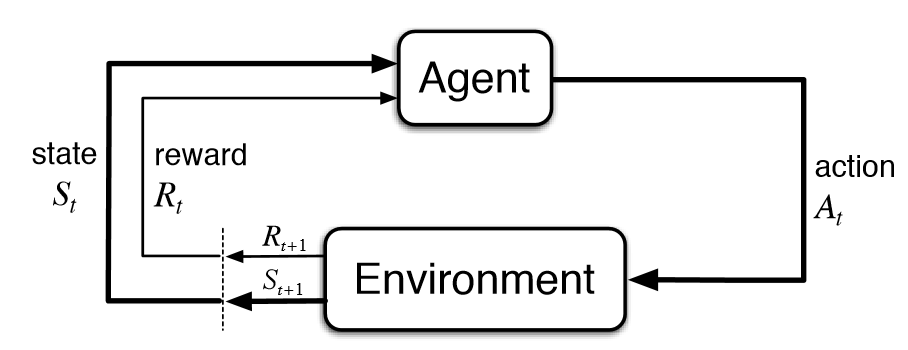
\includegraphics[scale=0.5]{img/RL_graph.png}
\vspace{1cm}

The agent's job is to find a behavior that maximizes the long-run sum of values of the rewards.
\end{frame}

\begin{frame}
\frametitle{Modelization}
\begin{block}{States}
States are defined in function of:
\begin{itemize}
\item distance to the traffic light
\item color of the traffic light
\item time spent seeing the color of the traffic light 
\item previous action 
\end{itemize}
\end{block}
\begin{block}{Speeds}
0,20,30,\ldots ,70
\end{block}
\end{frame}

\begin{frame}{}
\centering
\Huge{Thank you !} 
%\vspace{1cm}
\centering
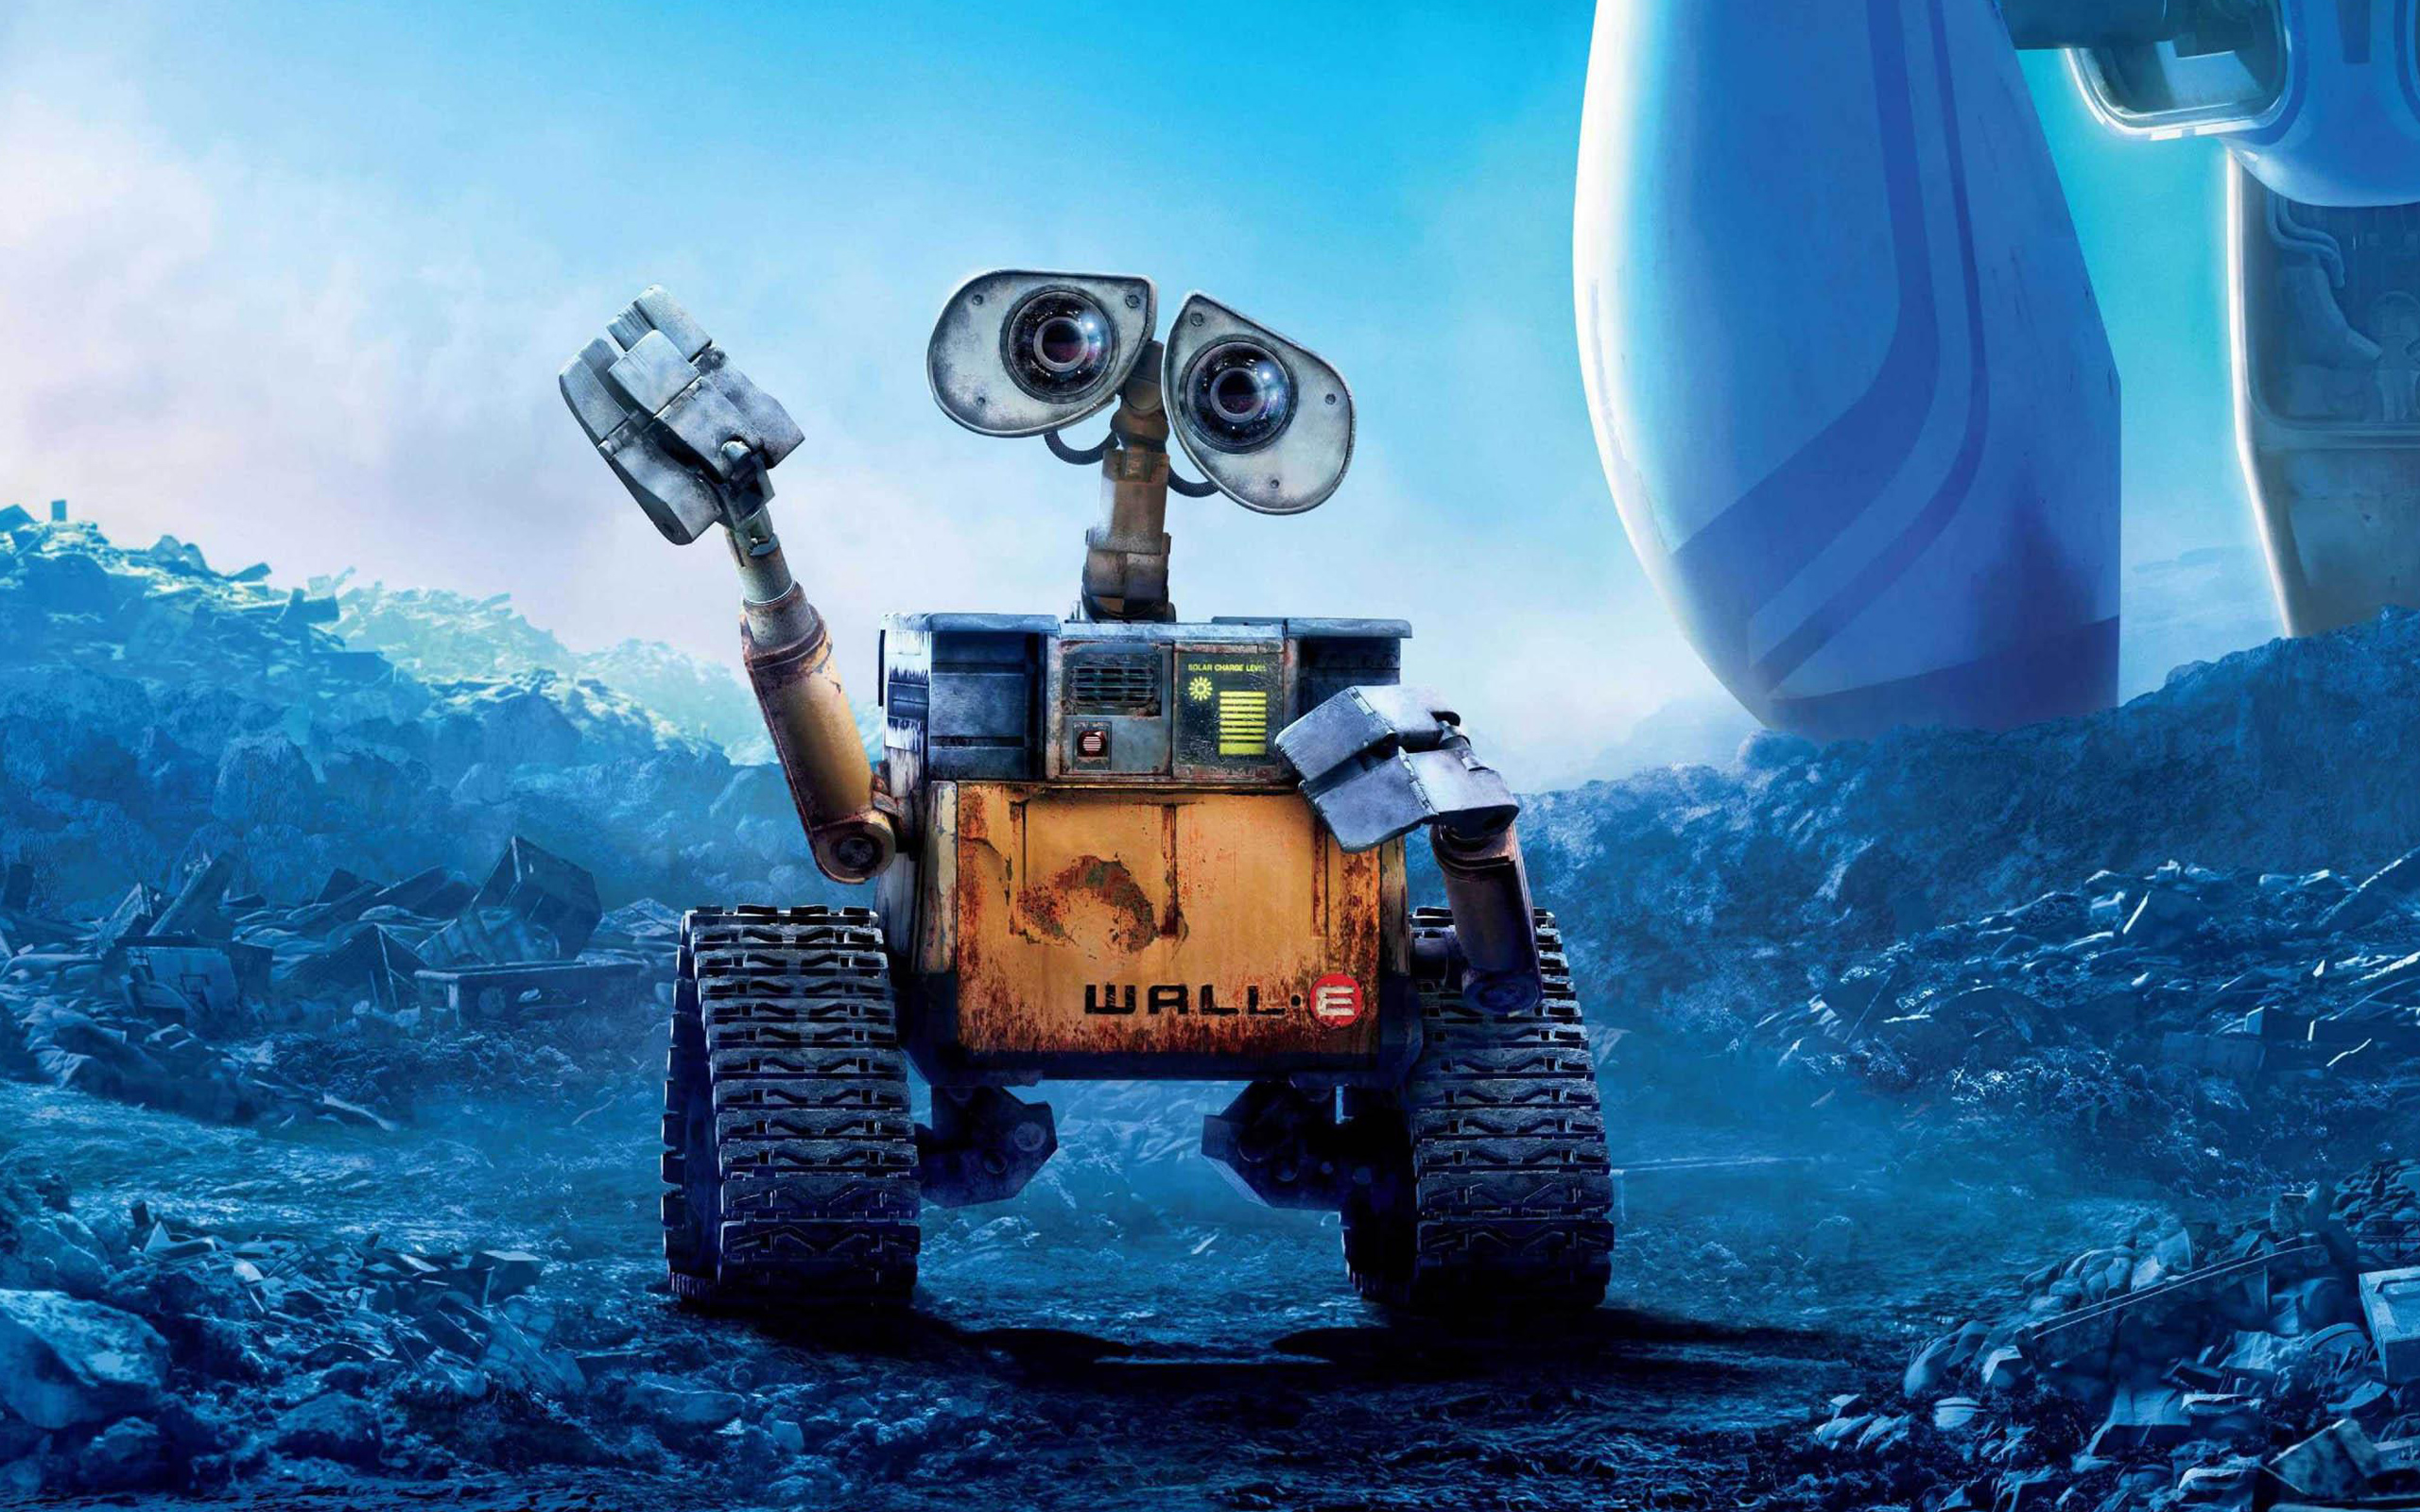
\includegraphics[scale=0.1]{img/walle_end.jpg}
\end{frame}




\end{document}
